\subsection{Agreement between data and simulation}
\label{sec:kpimm:data-mc}

Good agreement between data and simulated candidates is necessary in order to be able to accurately model the distortion of the angular distributions caused by the trigger, reconstruction and selection. The acceptance correction, described in detail in Sec.~\ref{sec:kpimm:acceptance}, is determined from simulated four-body \BdToKpimm decays generated according to a phase space distribution. Data driven techniques are used to improve the agreement between data and simulation. The PID distributions in simulation are corrected using a method known as `resampling'. To take into account remaining differences, simulated candidates are reweighted to match specific distributions in data.

\subsubsection{PID resampling}
\label{sec:kpimm:data-mc:resample}

Particle indentification information is used in two places within the selection of \BdToKpimm, for example to veto peaking backgrounds and as input to the multivariate classifier. The PID distributions are known to disagree between data and simulation. In order to improve the agreement, the distributions for each PID variable is resampled in a two stage process. Firstly, histograms of the PID variables are produced in bins of the number of tracks in the event, pseudorapidity and \pt using calibration samples in data. These samples include $\decay{\Dstarp}{\Dz(\to\Km\pip)\pim}$, $\decay{\Lz}{\proton\pim}$ and $\decay{\jpsi}{\mumu}$ decays. Secondly, the PID variables for simulated candidates are updated using the corresponding histogram as a PDF to draw a new value. This sampled value replaces the PID variable for the simulated candidate and is used in subsequent operations. The validation of the method for the variables \kaon\dllkpi and \pion\dllkpi is shown in Fig.~\ref{fig:kpimm:data-mc:pid} using sWeighted\footnote{A description of the \sPlot technique can be found in Ref.~\cite{splot}.} \BdToJPsiKst candidates in data and simulated \BdToJPsiKst candidates. The distributions for the remaining PID variables used in the candidate selection are shown in Appendix~\ref{sec:appendix:data-mc:pid}.

\begin{figure}[!tb]
 \centering
 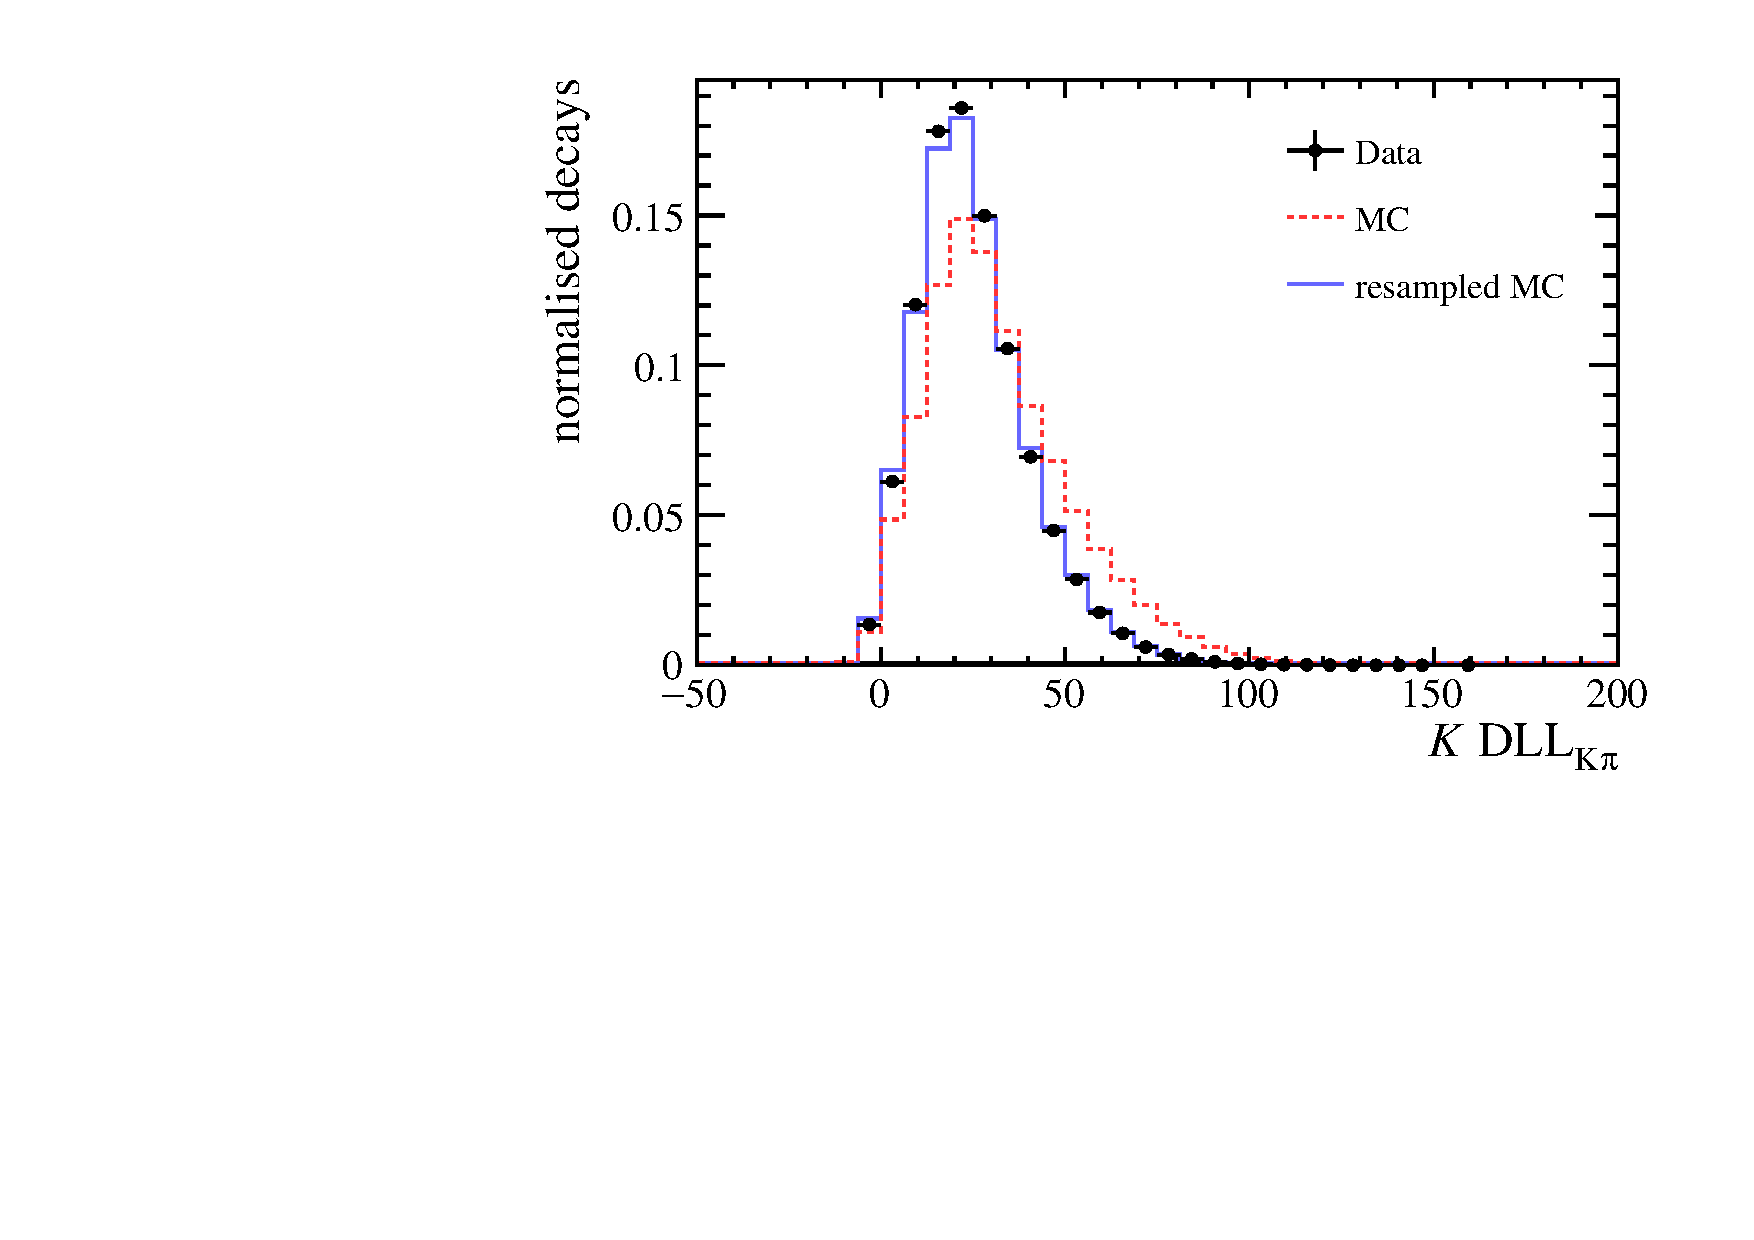
\includegraphics[width=0.49\textwidth]{figs/kpimm/data-mc/resampling/K_PIDK.pdf}
 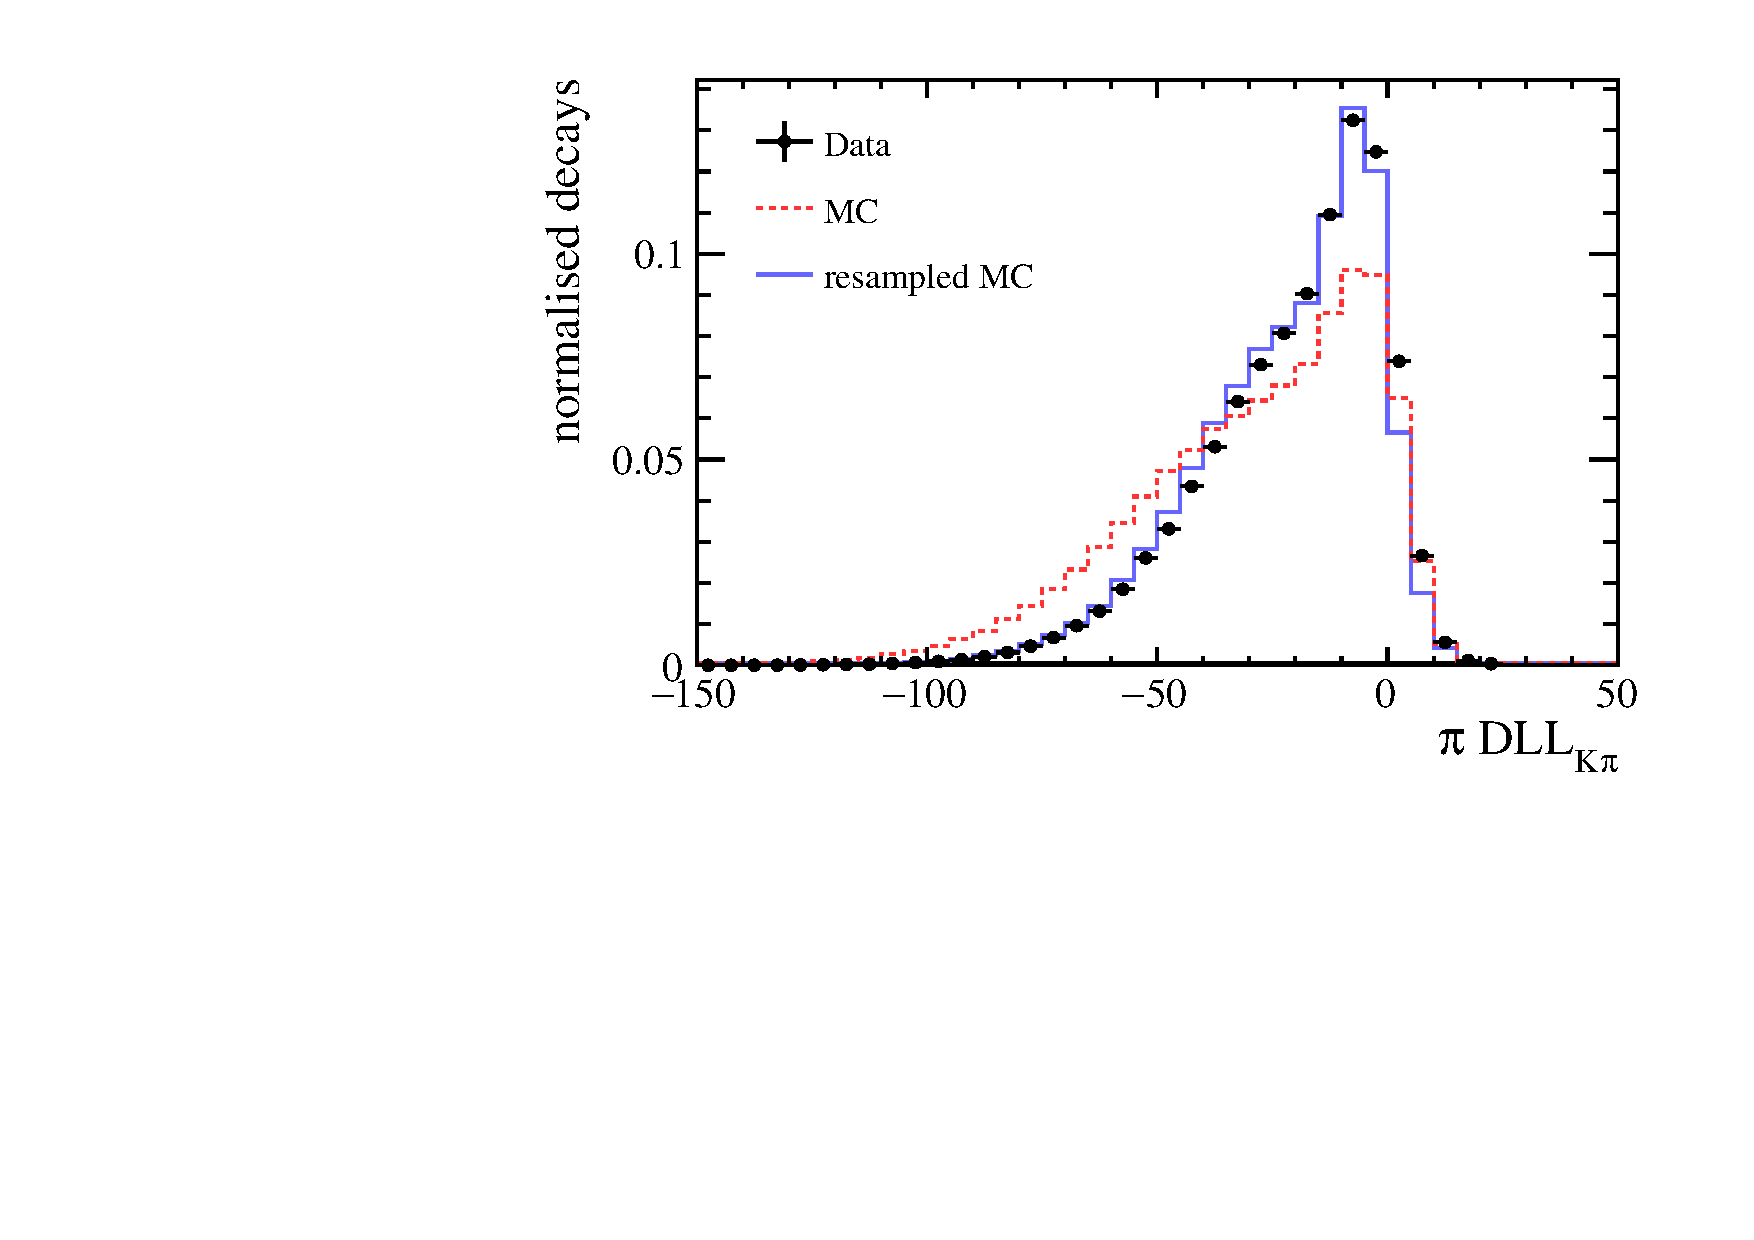
\includegraphics[width=0.49\textwidth]{figs/kpimm/data-mc/resampling/Pi_PIDK.pdf}
 \caption{Data-simulation agreement for the PID variables used in the selection of \BdToKpimm. The black data points show the distributions for sWeighted \BdToJPsiKst candidates in data. The red dashed histograms show the nominal distribution for simulated \BdToJPsiKst candidates. The blue histograms show the distribution for simulated \BdToJPsiKst candidates after the resampling procedure.}
\label{fig:kpimm:data-mc:pid}
\end{figure}

\subsubsection{Reweighting candidates to account for residual differences}
\label{sec:kpimm:data-mc:reweight}

The distribution of three variables that show differences between data and simulation are used to derive an candidate reweighting to improve agreement. These three variables are the following: the number of tracks in the event, the \pt of the \Bz candidate and the \Bz vertex quality $\chi^{2}$/ndof.
 
The candidate weights are derived by comparing sWeighted \BdToJPsiKst candidates in data and simulated \BdToJPsiKst candidates. 
%The candidates are required to be in the invariant mass ranges $796<\mkpi<996$~\mevcc and $9.22<\qsq<9.96$~\gevgevcccc. 
The weights are determined sequentially, with the previous weight being applied before the subsequent weight is derived. The candidate weights are then applied to all simulation samples. The validation of the method is shown in Fig.~\ref{fig:data-mc:reweight}. Figure~\ref{fig:data-mc:bdt} shows the agreement for the BDT response before and after applying the candidate reweighting.

\begin{figure}[!tb]
 \centering
 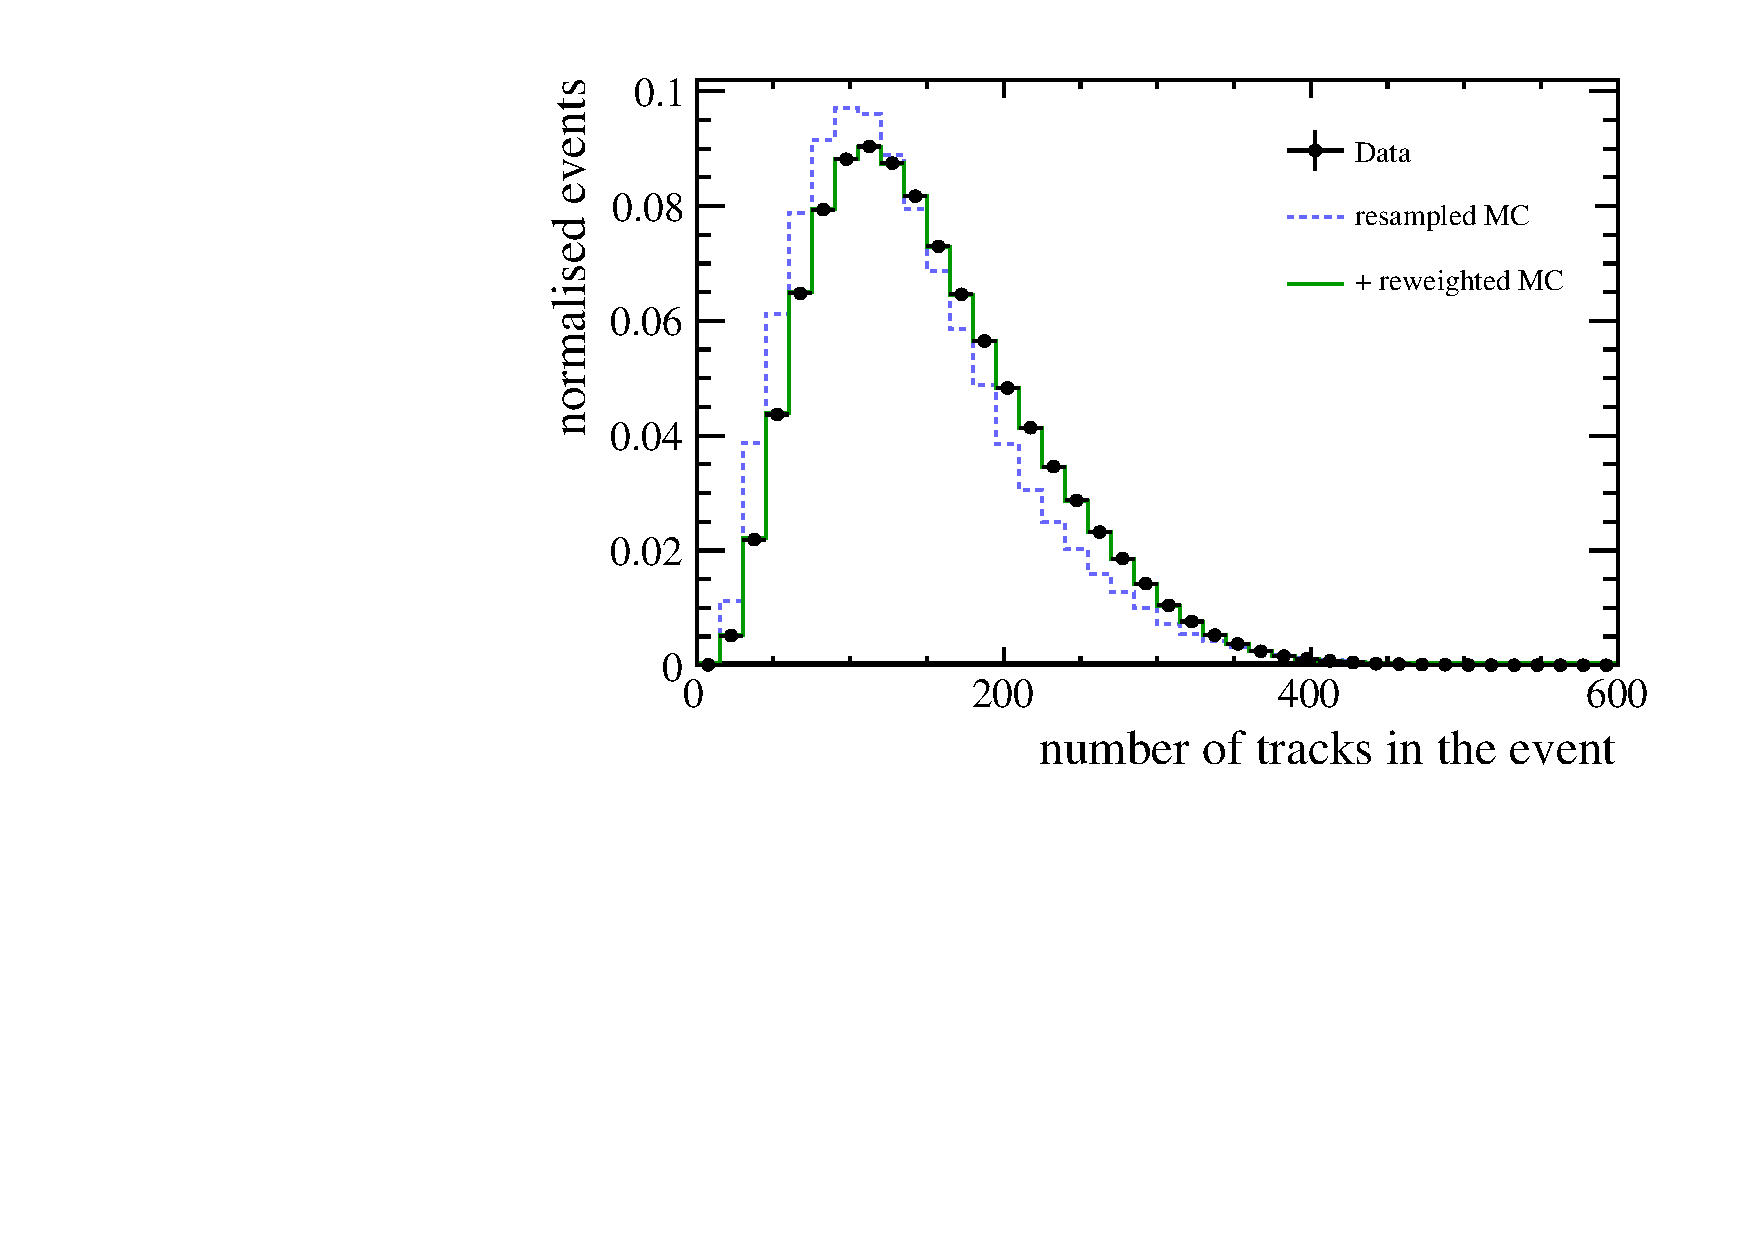
\includegraphics[width=0.49\textwidth]{figs/kpimm/data-mc/reweighting/nTracks.pdf}
 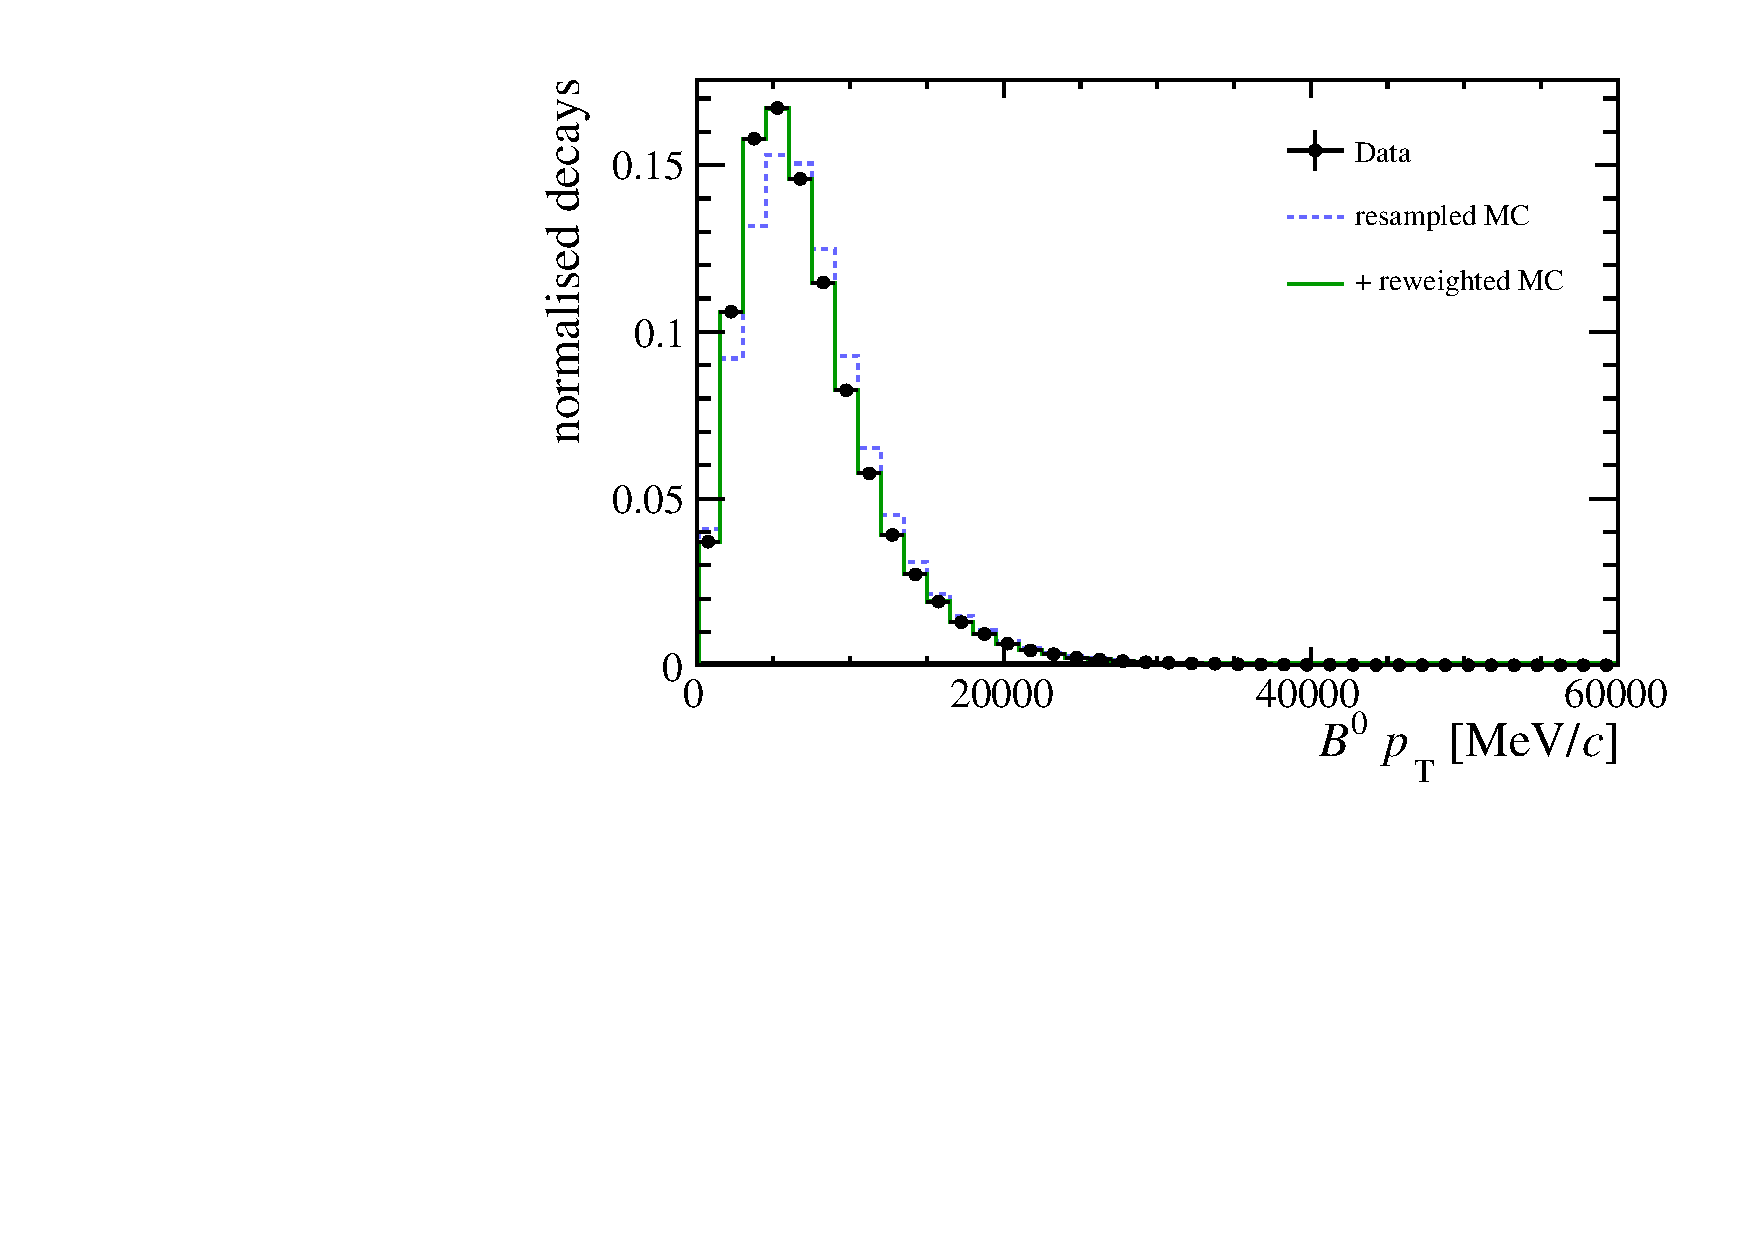
\includegraphics[width=0.49\textwidth]{figs/kpimm/data-mc/reweighting/B0_PT.pdf}
 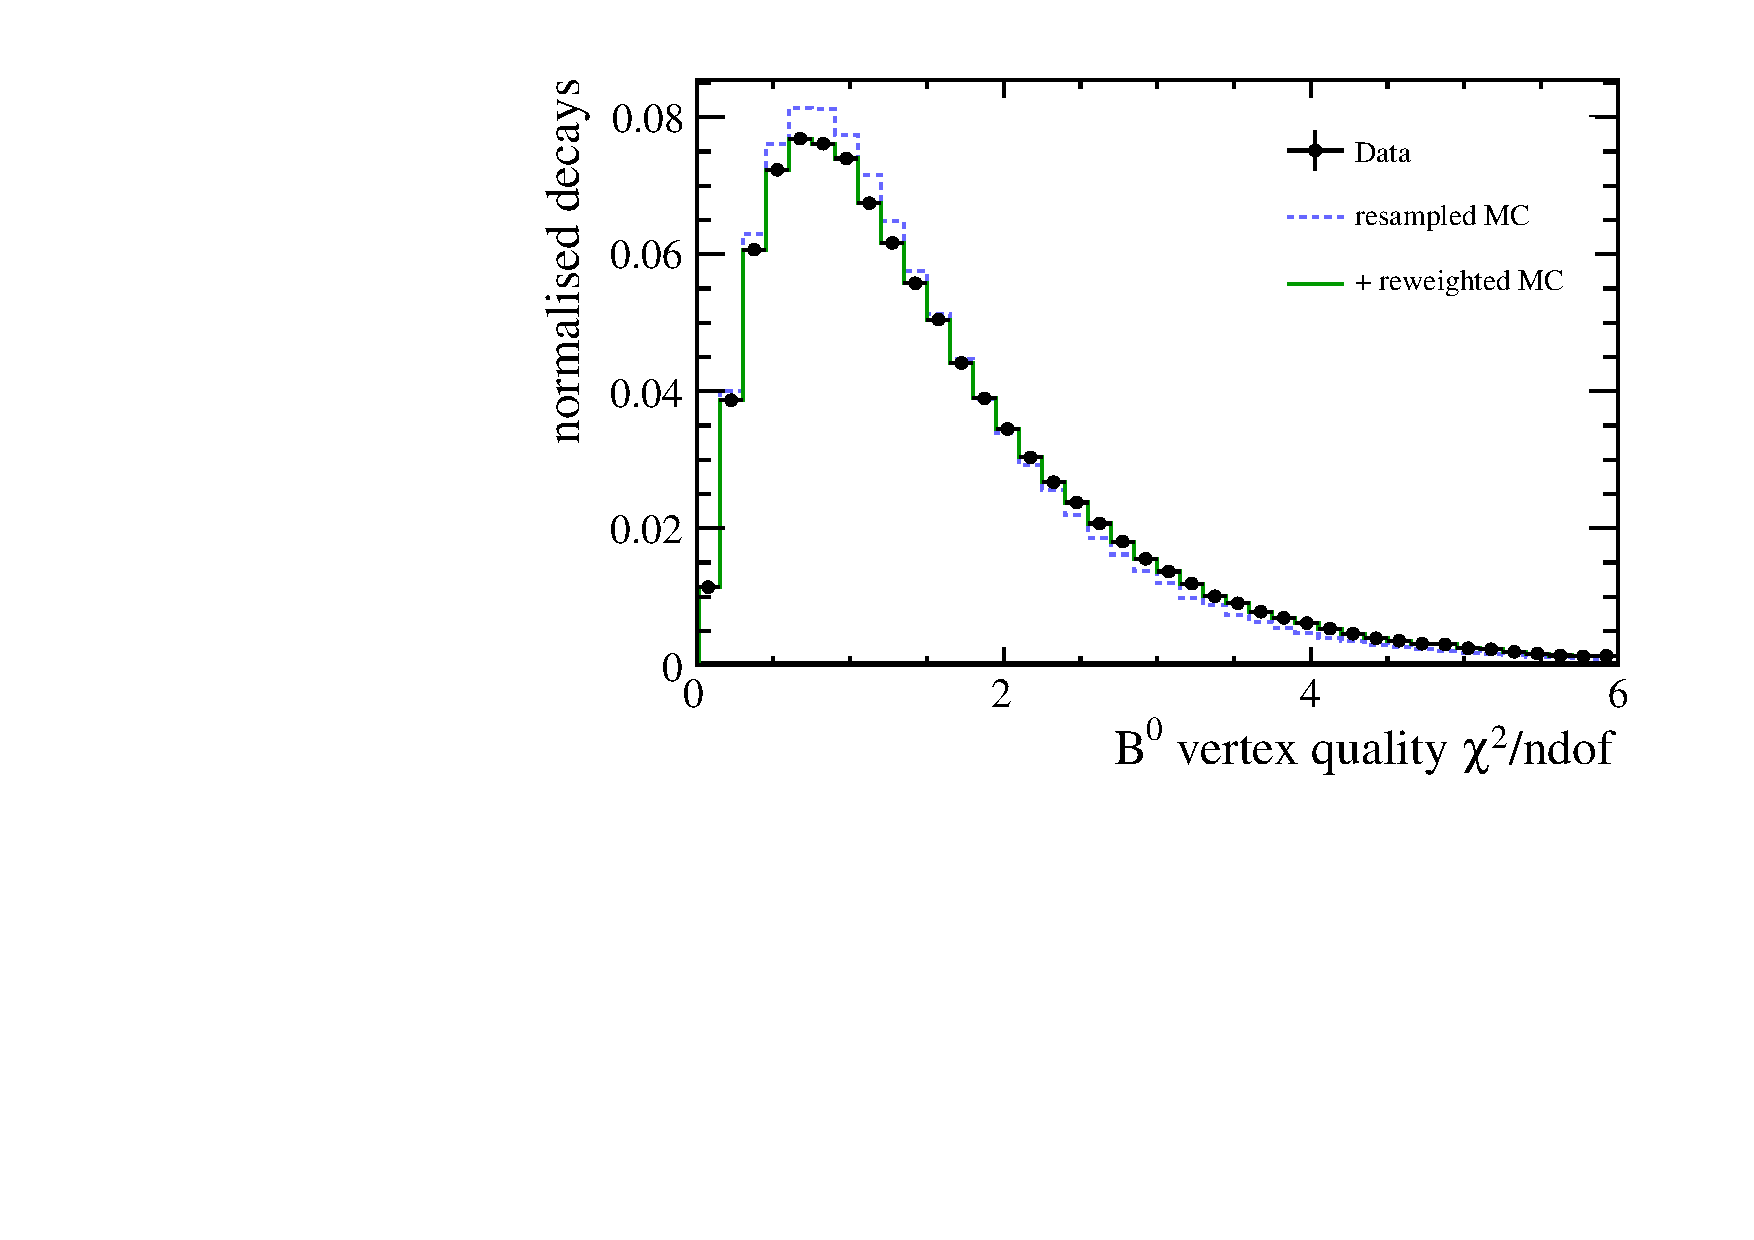
\includegraphics[width=0.49\textwidth]{figs/kpimm/data-mc/reweighting/B0_VertexChi2.pdf}
 
 \caption{Data-simulation agreement for the variables used to determine the candidate weights. The black data points show the distributions for sWeighted \BdToJPsiKst candidates in data. The blue dashed histograms show the distribution for resampled, simulated \BdToJPsiKst candidates. The green histograms show the distribution for resampled, simulated \BdToJPsiKst candidates with the candidate weights applied.}
 \label{fig:data-mc:reweight}
\end{figure}
 
\begin{figure}[!tb]
 \centering
 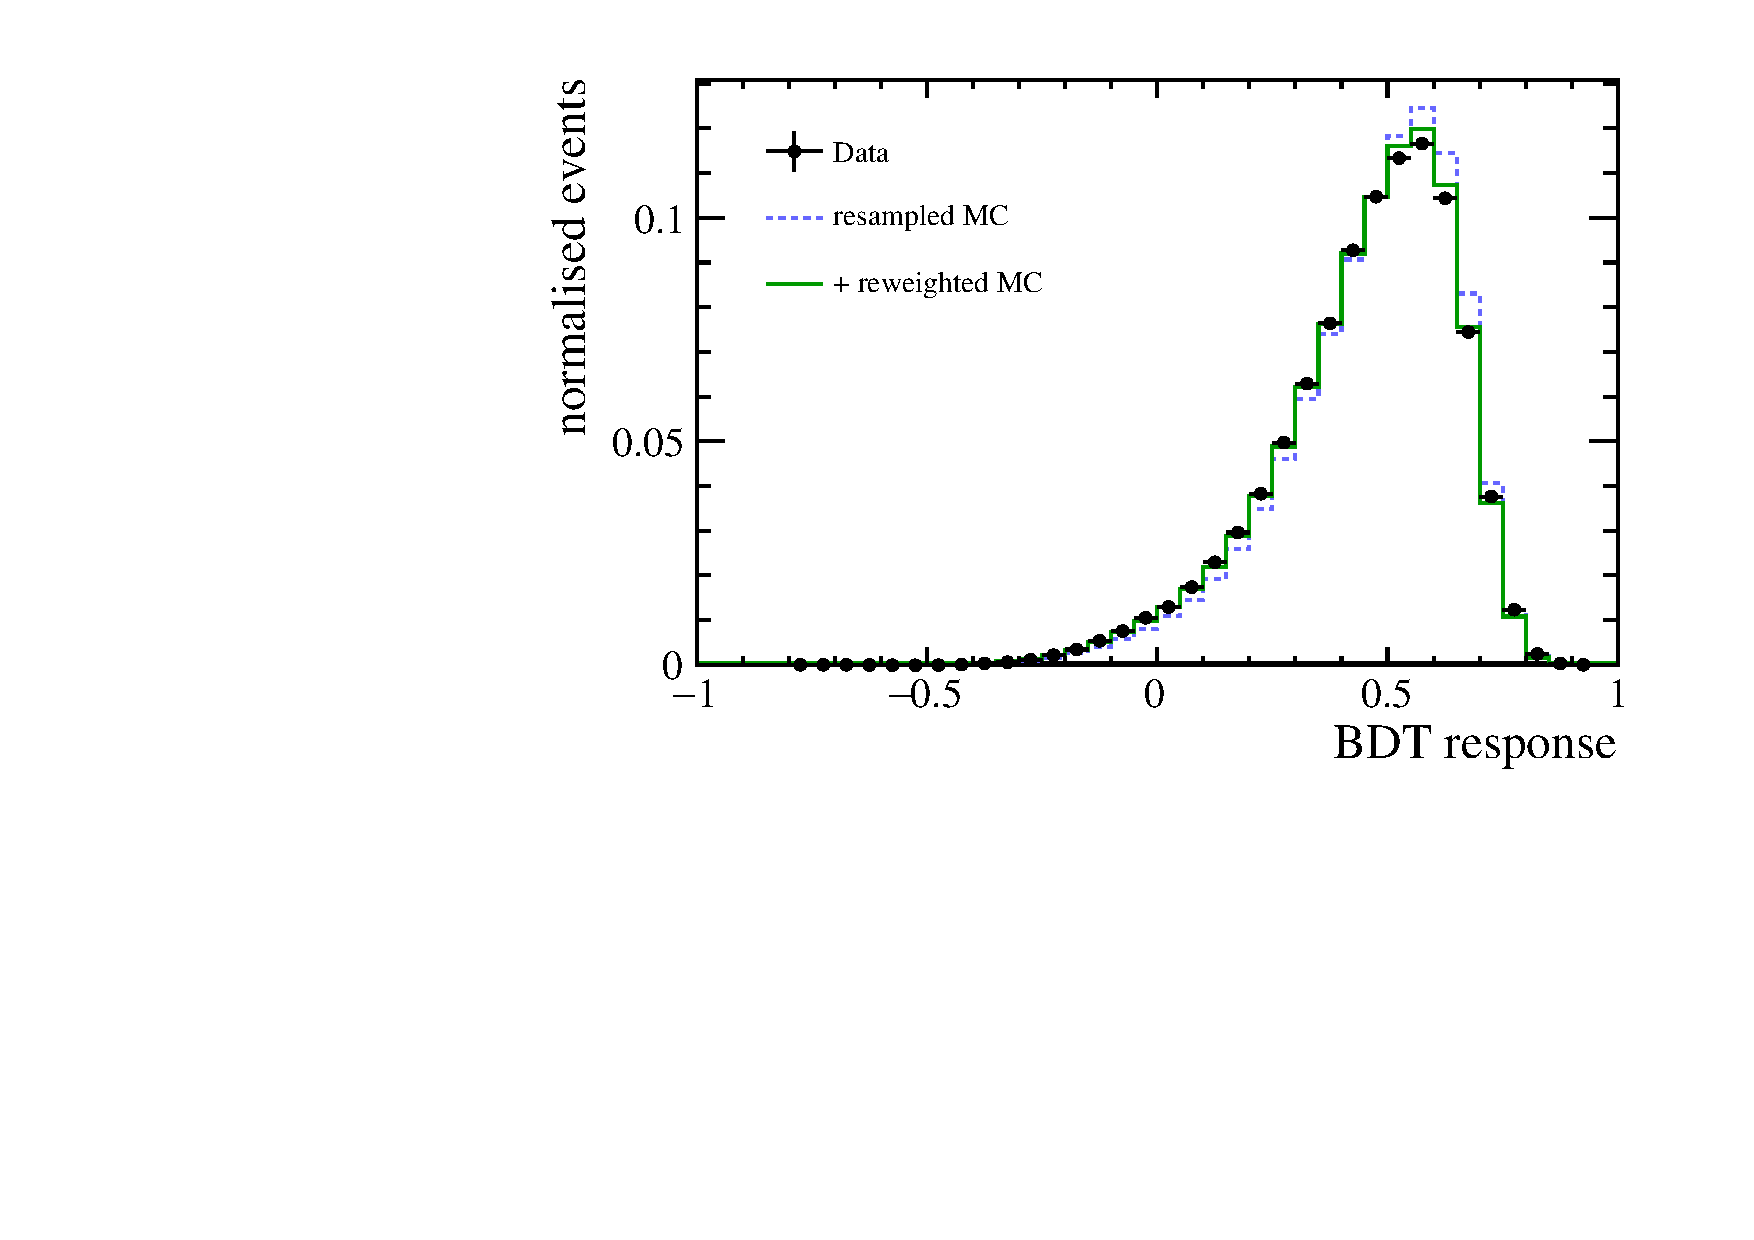
\includegraphics[width=0.7\textwidth]{figs/kpimm/data-mc/reweighting/BDT.pdf}
 
 \caption{Data-simulation agreement of the BDT response. The black data points show the distributions for sWeighted \BdToJPsiKst candidates in data. The blue dashed histograms show the distribution for resampled, simulated \BdToJPsiKst candidates. The green histograms show the distribution for resampled, simulated \BdToJPsiKst candidates with the candidate weights applied.}
\label{fig:data-mc:bdt}
\end{figure}